\documentclass{standalone}
\usepackage{pgfplots}

\begin{document}
	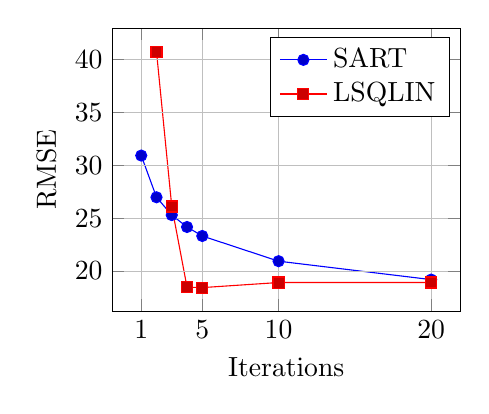
\begin{tikzpicture}
		
		\begin{axis}[	legend pos = north east, 
						legend cell align = left,
						xtick = {1, 5, 10, 20},
						ytick = {20, 25, 30, 35, 40},
						ylabel = {RMSE},
						xlabel = {Iterations},
						ylabel near ticks,
						grid = major,
						axis on top = true,
						width = 6 cm]
		
			%% NOTE: I multiplied by 1 / sqrt(3) because I forgot to normalize the MSE by the number of color channels.
		
			\addplot coordinates {
				(1, 53.517116 * 0.5774)
				(2, 46.6983 * 0.5774)
				(3, 43.7923 * 0.5774)
				(4, 41.8413 * 0.5774)
				(5, 40.3709 * 0.5774)
				(10, 36.2524 * 0.5774)
				(20, 33.2420 * 0.5774)
			};
			\addlegendentry{SART};
			
			\addplot coordinates {
				(2, 70.477447 * 0.5774)
				(3, 45.188843 * 0.5774)
				(4, 32.001308 * 0.5774)
				(5, 31.934515 * 0.5774)
				(10, 32.764468 * 0.5774)
				(20, 32.766828 * 0.5774)
			};
			\addlegendentry{LSQLIN};
			
			 
		\end{axis}
		
	\end{tikzpicture}
\end{document}